
The face detection part of our algorithm performs flawlessly on the original images in the given dataset which can be seen in Figure \ref{fig:faces} as most outputs from the images in the given dataset is included in it. That it performs well on these original images is not a coincidence as the algorithm was developed and verified through testing on the given datasets. In Figure \ref{fig:fdResults} we showcase how tolerant our algorithm can be for various conditions in certain images.

\begin{figure}[H]
\centering

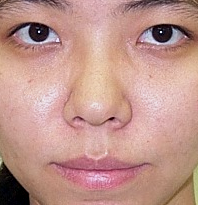
\includegraphics[width=0.09\textwidth]{img/fdResult1/output3.png}
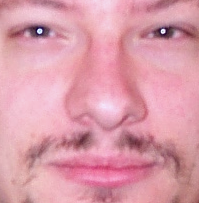
\includegraphics[width=0.09\textwidth]{img/fdResult1/output4.png}
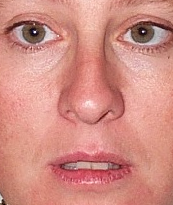
\includegraphics[width=0.09\textwidth]{img/fdResult1/output9.png}
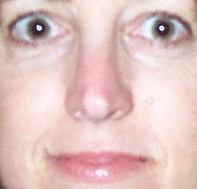
\includegraphics[width=0.09\textwidth]{img/fdResult1/output12.png}
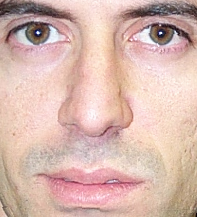
\includegraphics[width=0.09\textwidth]{img/fdResult1/output14.png}
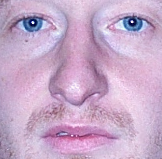
\includegraphics[width=0.09\textwidth]{img/fdResult1/output15.png}
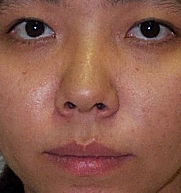
\includegraphics[width=0.09\textwidth]{img/fdResult1/output16.png}
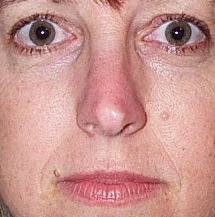
\includegraphics[width=0.09\textwidth]{img/fdResult1/output17.png}
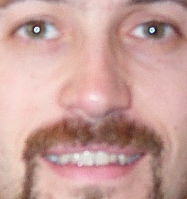
\includegraphics[width=0.09\textwidth]{img/fdResult1/output18.png}
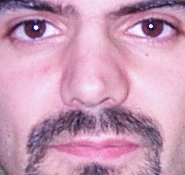
\includegraphics[width=0.09\textwidth]{img/fdResult1/output27.png}
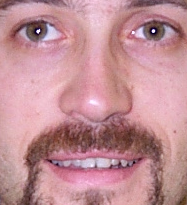
\includegraphics[width=0.09\textwidth]{img/fdResult1/output28.png}
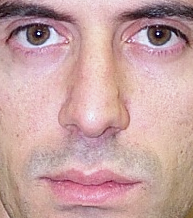
\includegraphics[width=0.09\textwidth]{img/fdResult1/output32.png}
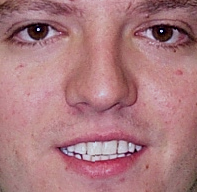
\includegraphics[width=0.09\textwidth]{img/fdResult1/output38.png}
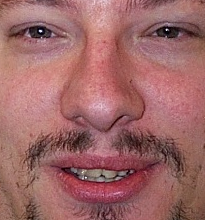
\includegraphics[width=0.09\textwidth]{img/fdResult1/output39.png}
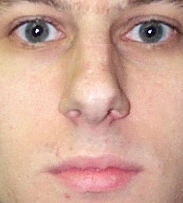
\includegraphics[width=0.09\textwidth]{img/fdResult1/output42.png}
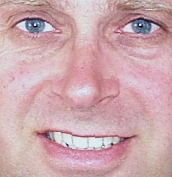
\includegraphics[width=0.09\textwidth]{img/fdResult1/output44.png}
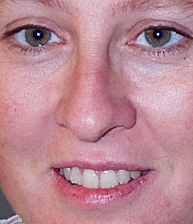
\includegraphics[width=0.09\textwidth]{img/fdResult1/output45.png}
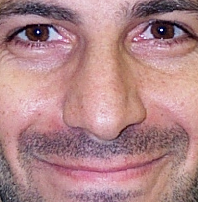
\includegraphics[width=0.09\textwidth]{img/fdResult1/output49.png}
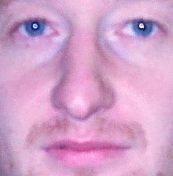
\includegraphics[width=0.09\textwidth]{img/fdResult1/output50.png}
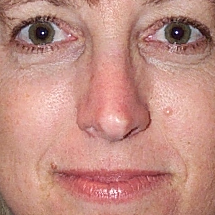
\includegraphics[width=0.09\textwidth]{img/fdResult1/output55.png}
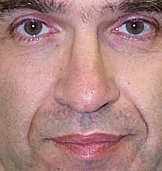
\includegraphics[width=0.09\textwidth]{img/fdResult1/output63.png}
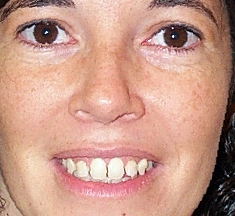
\includegraphics[width=0.09\textwidth]{img/fdResult1/output65.png}
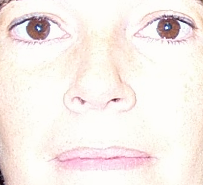
\includegraphics[width=0.09\textwidth]{img/fdResult1/output66.png}
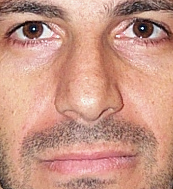
\includegraphics[width=0.09\textwidth]{img/fdResult1/output68.png}
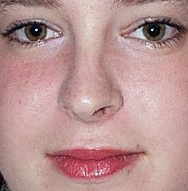
\includegraphics[width=0.09\textwidth]{img/fdResult1/output70.png}
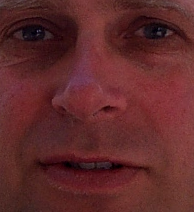
\includegraphics[width=0.09\textwidth]{img/fdResult1/output71.png}
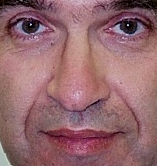
\includegraphics[width=0.09\textwidth]{img/fdResult1/output75.png}
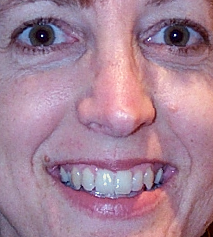
\includegraphics[width=0.09\textwidth]{img/fdResult1/output76.png}
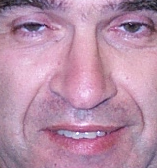
\includegraphics[width=0.09\textwidth]{img/fdResult1/output77.png}
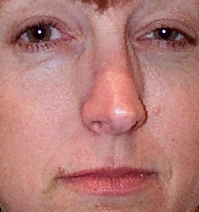
\includegraphics[width=0.09\textwidth]{img/fdResult1/output80.png}
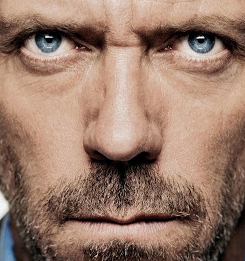
\includegraphics[width=0.09\textwidth]{img/fdResult2/output9.png}
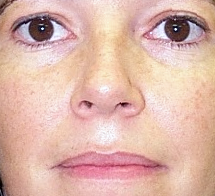
\includegraphics[width=0.09\textwidth]{img/fdResult1/output83.png}
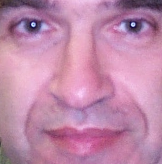
\includegraphics[width=0.09\textwidth]{img/fdResult1/output85.png}
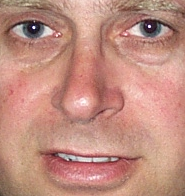
\includegraphics[width=0.09\textwidth]{img/fdResult1/output91.png}
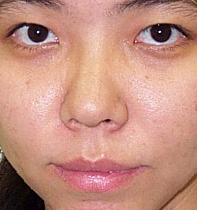
\includegraphics[width=0.09\textwidth]{img/fdResult1/output92.png}
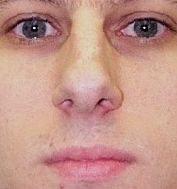
\includegraphics[width=0.09\textwidth]{img/fdResult1/output95.png}
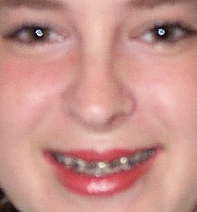
\includegraphics[width=0.09\textwidth]{img/fdResult1/output96.png}
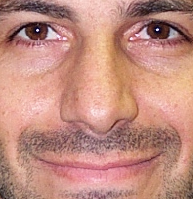
\includegraphics[width=0.09\textwidth]{img/fdResult1/output97.png}
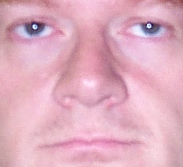
\includegraphics[width=0.09\textwidth]{img/fdResult1/output98.png}
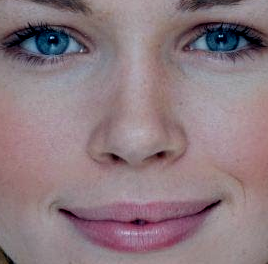
\includegraphics[width=0.09\textwidth]{img/fdResult2/output91.png}

\caption{Successful experimental results of face detection.}
\label{fig:faces}
\end{figure}

% \begin{figure}[H]
\centering

\begin{subfigure}{.25\textwidth}
  \centering
  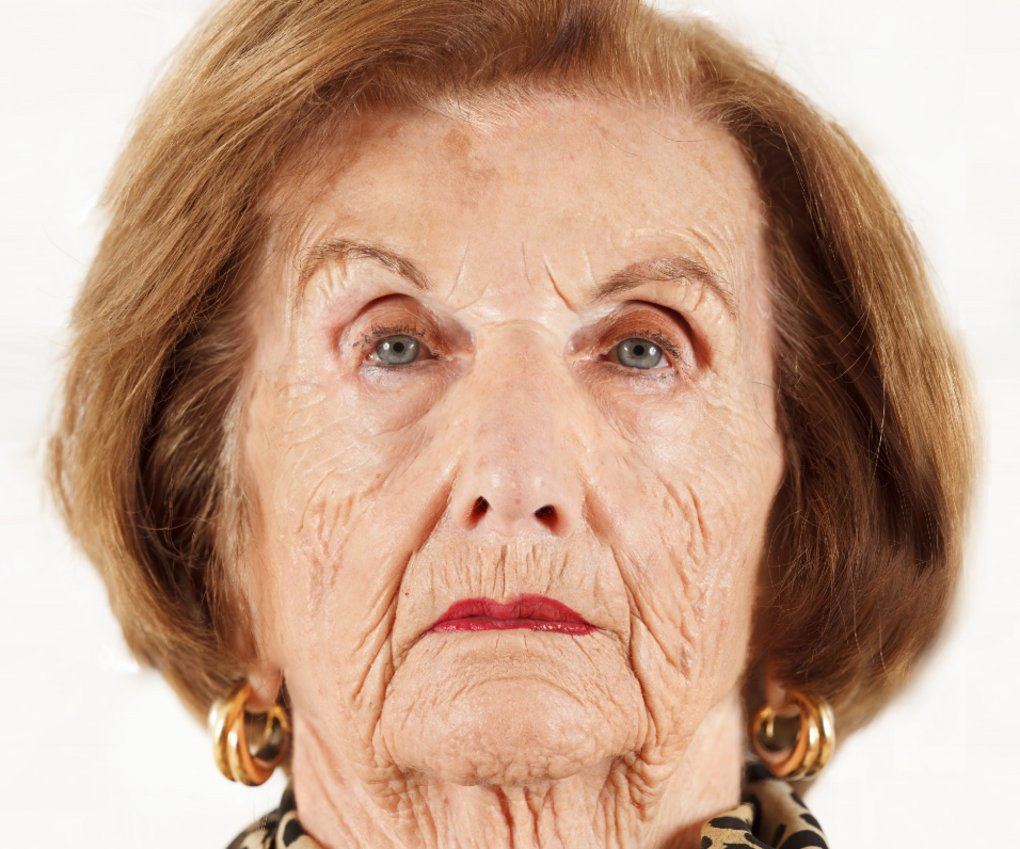
\includegraphics[width=0.95\textwidth]{img/fd3/fail1_input.jpg}
  \caption{}
\end{subfigure}%
\begin{subfigure}{.25\textwidth}
  \centering
  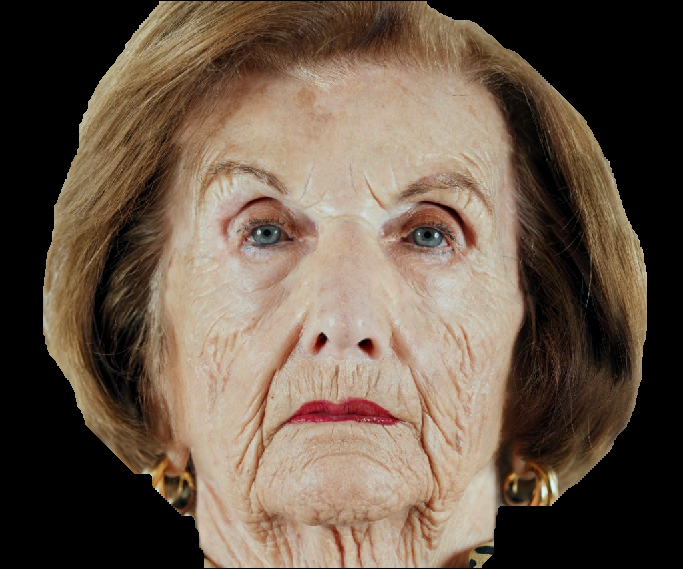
\includegraphics[width=0.95\textwidth]{img/fd3/fail1_faceImage.png}
  \caption{}
\end{subfigure}%
\begin{subfigure}{.25\textwidth}
  \centering
  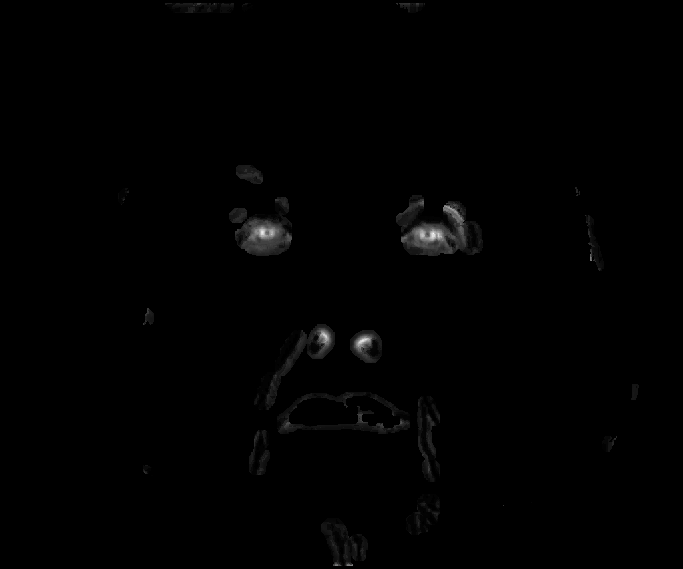
\includegraphics[width=0.95\textwidth]{img/fd3/fail1_finalEyeMap.png}
  \caption{}
\end{subfigure}%
\begin{subfigure}{.25\textwidth}
  \centering
  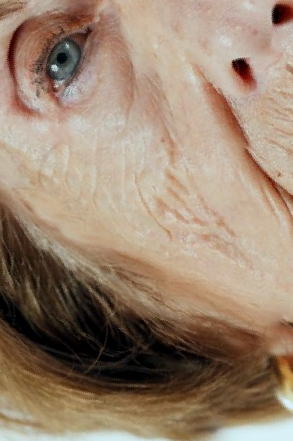
\includegraphics[width=0.53\textwidth]{img/fd3/fail1_output.png}
  \caption{}
\end{subfigure}%

\caption{Resonera, Fail1}
\label{fig:fail1}
\end{figure}


\begin{figure}[H]
\centering

\begin{subfigure}{.25\textwidth}
  \centering
  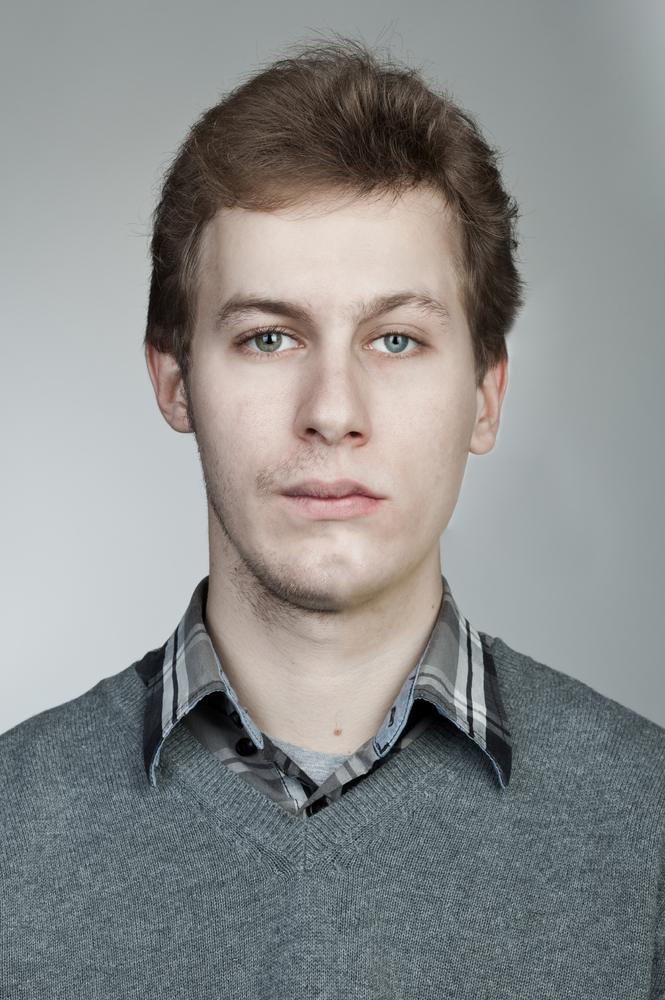
\includegraphics[width=0.53\textwidth]{img/fd3/fail2_input.jpg}
  \caption{}
\end{subfigure}%
\begin{subfigure}{.25\textwidth}
  \centering
  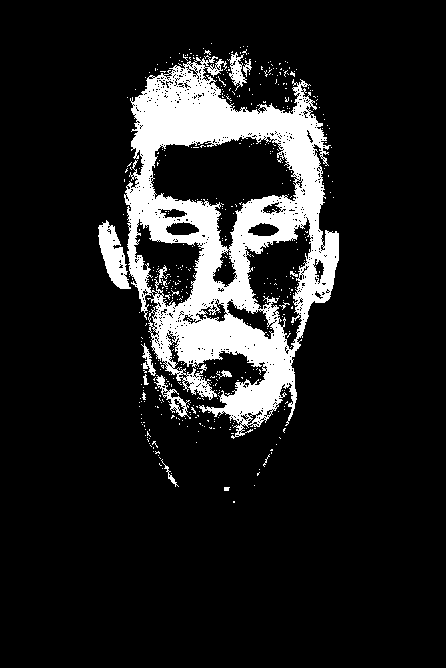
\includegraphics[width=0.53\textwidth]{img/fd3/fail2_estimatedSkinMak.png}
  \caption{}
\end{subfigure}%
\begin{subfigure}{.25\textwidth}
  \centering
  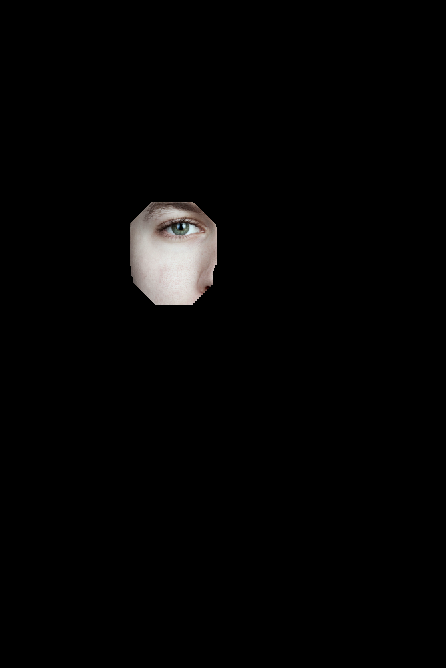
\includegraphics[width=0.53\textwidth]{img/fd3/fail2_faceImage.png}
  \caption{}
\end{subfigure}%
\begin{subfigure}{.25\textwidth}
  \centering
  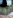
\includegraphics[width=0.23\textwidth]{img/fd3/fail2_output.png}
  \caption{}
\end{subfigure}%

\caption{Resonera, Fail2}
\label{fig:fail2}
\end{figure}




\begin{figure}[H]
\centering

\begin{subfigure}{.25\textwidth}
  \centering
  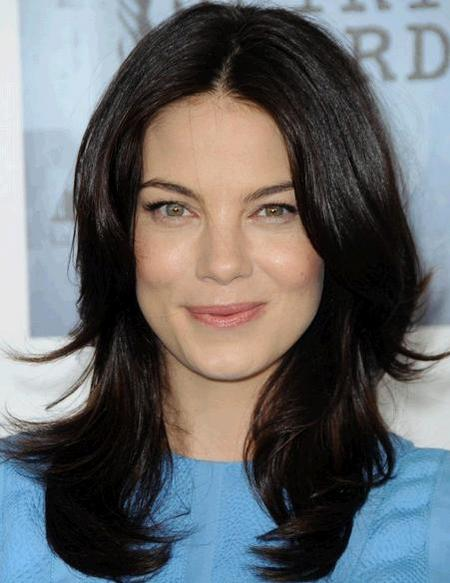
\includegraphics[width=0.53\textwidth]{img/fd3/fail3_input.jpg}
  \caption{}
\end{subfigure}%
\begin{subfigure}{.25\textwidth}
  \centering
  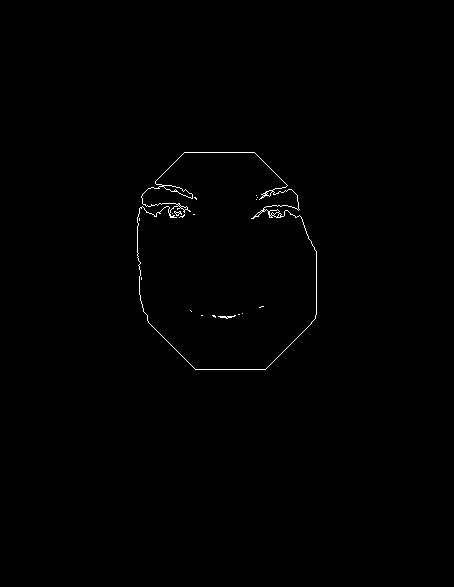
\includegraphics[width=0.53\textwidth]{img/fd3/fail3_faceBorder.png}
  \caption{}
\end{subfigure}%
\begin{subfigure}{.25\textwidth}
  \centering
  \includegraphics[width=0.53\textwidth]{img/fd3/fail3_eyeCandidates.png}
  \caption{}
\end{subfigure}%
% \begin{subfigure}{.15\textwidth}
%   \centering
%   \includegraphics[width=0.53\textwidth]{img/fd3/fail3_faceImage.png}
%   \caption{}
% \end{subfigure}%
% \begin{subfigure}{.15\textwidth}
%   \centering
%   \includegraphics[width=0.53\textwidth]{img/fd3/fail3_finalEyeMap.png}
%   \caption{}
% \end{subfigure}%
\begin{subfigure}{.25\textwidth}
  \centering
  \includegraphics[width=0.23\textwidth]{img/fd3/fail3_output.png}
  \caption{}
\end{subfigure}%

\caption{Resonera, Fail3}
\label{fig:fail3}
\end{figure}




\begin{figure}[H]
\centering

\begin{subfigure}{.25\textwidth}
  \centering
  \includegraphics[width=0.95\textwidth]{img/fd3/fail4_input.jpg}
  \caption{}
\end{subfigure}%
\begin{subfigure}{.25\textwidth}
  \centering
  \includegraphics[width=0.95\textwidth]{img/fd3/fail4_faceBorder.png}
  \caption{}
\end{subfigure}%
\begin{subfigure}{.25\textwidth}
  \centering
  \includegraphics[width=0.95\textwidth]{img/fd3/fail4_eyeCandidates.png}
  \caption{}
\end{subfigure}%
% \begin{subfigure}{.15\textwidth}
%   \centering
%   \includegraphics[width=0.95\textwidth]{img/fd3/fail4_faceImage.png}
%   \caption{}
% \end{subfigure}%
% \begin{subfigure}{.15\textwidth}
%   \centering
%   \includegraphics[width=0.95\textwidth]{img/fd3/fail4_finalEyeMap.png}
%   \caption{}
% \end{subfigure}%
\begin{subfigure}{.25\textwidth}
  \centering
  \includegraphics[width=0.53\textwidth]{img/fd3/fail4_output.png}
  \caption{}
\end{subfigure}%

\caption{Resonera, Fail4}
\label{fig:fail4}
\end{figure}









However when our algorithm is faced with tougher conditions, for example blurry  or very small images it somewhat breaks down. Examples of failed face detection can be seen in Figure \ref{fig:fail1} and \ref{fig:fail3}. This is presumably due to hard coded thresholds and kernel widths for the morphological operations as well as for the methods themselves, especially the part were we derive the eye candidates. Detailed results where we have made the images harder to analyze through adding artificial artifacts can be looked up in Table \ref{tb:result}.

\begin{figure}[H]
\centering

\begin{subfigure}{.25\textwidth}
  \centering
  \includegraphics[width=0.95\textwidth]{img/fd3/fail1_input.jpg}
  \caption{}
\end{subfigure}%
\begin{subfigure}{.25\textwidth}
  \centering
  \includegraphics[width=0.95\textwidth]{img/fd3/fail1_faceImage.png}
  \caption{}
\end{subfigure}%
\begin{subfigure}{.25\textwidth}
  \centering
  \includegraphics[width=0.95\textwidth]{img/fd3/fail1_finalEyeMap.png}
  \caption{}
\end{subfigure}%
\begin{subfigure}{.25\textwidth}
  \centering
  \includegraphics[width=0.53\textwidth]{img/fd3/fail1_output.png}
  \caption{}
\end{subfigure}%

\caption{A case where the proposed algorithm fails to detect the correct face due to an invalid extraction of the eyes from the eye map. (a) show the input image, (b) the correctly extracted face mask, (c) the proper eye map while (d) show the output image where the extraction of the eyes using the Circular Hough Transform fail by mixing up the left nostril with the right eye. }
\label{fig:fail1}
\end{figure}







\begin{figure}[H]
\centering

\begin{subfigure}{.25\textwidth}
  \centering
  \includegraphics[width=0.53\textwidth]{img/fd3/fail3_input.jpg}
  \caption{}
\end{subfigure}%
\begin{subfigure}{.25\textwidth}
  \centering
  \includegraphics[width=0.53\textwidth]{img/fd3/fail3_faceBorder.png}
  \caption{}
\end{subfigure}%
\begin{subfigure}{.25\textwidth}
  \centering
  \includegraphics[width=0.53\textwidth]{img/fd3/fail3_eyeCandidates.png}
  \caption{}
\end{subfigure}%
% \begin{subfigure}{.15\textwidth}
%   \centering
%   \includegraphics[width=0.53\textwidth]{img/fd3/fail3_faceImage.png}
%   \caption{}
% \end{subfigure}%
% \begin{subfigure}{.15\textwidth}
%   \centering
%   \includegraphics[width=0.53\textwidth]{img/fd3/fail3_finalEyeMap.png}
%   \caption{}
% \end{subfigure}%
\begin{subfigure}{.25\textwidth}
  \centering
  \includegraphics[width=0.23\textwidth]{img/fd3/fail3_output.png}
  \caption{}
\end{subfigure}%

\caption{A case where the proposed algorithm fails to detect the correct face due to a lack of eye candidates for both eyes. (a) show the input image, (b) the filtered face mask that gives the insufficient eye candidates in (c) and lead to the invalid output (d).}
\label{fig:fail3}
\end{figure}


\begin{figure}[H]
\centering

\begin{subfigure}{0.65\textwidth}
\begin{subfigure}{.33\textwidth}
  \centering
  \includegraphics[width=0.95\textwidth]{img/fdResult1/input63.png}
  \caption{}
\end{subfigure}%
\begin{subfigure}{.33\textwidth}
  \centering
  \includegraphics[width=0.6\textwidth]{img/fdResult1/output63.png}
  \caption{}
\end{subfigure}%
\end{subfigure}%
\begin{subfigure}{0.65\textwidth}
\begin{subfigure}{.33\textwidth}
  \centering
  \includegraphics[width=0.95\textwidth]{img/fdResult1/input18.png}
  \caption{}
\end{subfigure}%
\begin{subfigure}{.33\textwidth}
  \centering
  \includegraphics[width=0.6\textwidth]{img/fdResult1/output18.png}
  \caption{}
\end{subfigure}%
\end{subfigure}%

\begin{subfigure}{0.65\textwidth}
\begin{subfigure}{.33\textwidth}
  \centering
  \includegraphics[width=0.95\textwidth]{img/fdResult2/input12.png}
  \caption{}
\end{subfigure}%
\begin{subfigure}{.33\textwidth}
  \centering
  \includegraphics[width=0.6\textwidth]{img/fdResult2/output12.png}
  \caption{}
\end{subfigure}%
\end{subfigure}%
\begin{subfigure}{0.65\textwidth}
\begin{subfigure}{.33\textwidth}
  \centering
  \includegraphics[width=0.95\textwidth]{img/fdResult2/input92.png}
  \caption{}
\end{subfigure}%
\begin{subfigure}{.33\textwidth}
  \centering
  \includegraphics[width=0.6\textwidth]{img/fdResult2/output92.png}
  \caption{}
\end{subfigure}%
\end{subfigure}%

\begin{subfigure}{0.65\textwidth}
\begin{subfigure}{.33\textwidth}
  \centering
  \includegraphics[width=0.95\textwidth]{img/fdResult2/input63.png}
  \caption{}
\end{subfigure}%
\begin{subfigure}{.33\textwidth}
  \centering
  \includegraphics[width=0.6\textwidth]{img/fdResult2/output63.png}
  \caption{}
\end{subfigure}%
\end{subfigure}%
\begin{subfigure}{0.65\textwidth}
\begin{subfigure}{.33\textwidth}
  \centering
  \includegraphics[width=0.95\textwidth]{img/fdResult2/input82.png}
  \caption{}
\end{subfigure}%
\begin{subfigure}{.33\textwidth}
  \centering
  \includegraphics[width=0.6\textwidth]{img/fdResult2/output82.png}
  \caption{}
\end{subfigure}%
\end{subfigure}%

\begin{subfigure}{0.65\textwidth}
\begin{subfigure}{.33\textwidth}
  \centering
  \includegraphics[width=0.95\textwidth]{img/fdResult1/input66.png}
  \caption{}
\end{subfigure}%
\begin{subfigure}{.33\textwidth}
  \centering
  \includegraphics[width=0.6\textwidth]{img/fdResult1/output66.png}
  \caption{}
\end{subfigure}%
\end{subfigure}%
\begin{subfigure}{0.65\textwidth}
\begin{subfigure}{.33\textwidth}
  \centering
  \includegraphics[width=0.95\textwidth]{img/fdResult1/input76.png}
  \caption{}
\end{subfigure}%
\begin{subfigure}{.33\textwidth}
  \centering
  \includegraphics[width=0.6\textwidth]{img/fdResult1/output76.png}
  \caption{}
\end{subfigure}%
\end{subfigure}%

\caption{Results of the face detection phase depicting the algorithm's tolerance for varying environments \textit{(a-d)}, lightning conditions \textit{(e-h, m-p)}, poses \textit{(i-j)} and amount of skin color in the image \textit{(c-d, k-l)}.}


\label{fig:fdResults}
\end{figure}


\begin{table}[H]
\small
  \captionof{table}{The resulting hit ratios over all images for different test scenarios.}
  \label{tb:result}
\begin{tabular}{l*{10}{c}r}
\hline
Parameters & Access (db1) & No access (db0) & Hard (db2) & Test images \\
\hline
Blur, $\sigma$ = 0.5  & 94\% 	& 75\% 		& 95\% 		& 50\%  \\ \hline
Blur, $\sigma$ = 1.0  & 88\% 		& 50\% 		& 84\% 	& 50\% \\ \hline
Blur, $\sigma$ = 2.5  & 19\% 	& 25\% 		& 84\% 		& 33\% \\ \hline
Tone, I = 0.5  		& 94\% 	& 100\%	 		& 95\%		& 94\% \\ \hline
Tone, I = 0.7  		& 94\%		& 100\%   	    & 95\% 	& 89\% 	\\ \hline
Tone, I = 1.3  		& 75\%		& 75\%		& 87\% 	& 61\% 	 \\ \hline
Scale, s = 0.9 		& 100\% 		& 50\% 		& 95\% 	& 94\% 	 \\ \hline
Scale, s = 1.1  		& 100\% 		& 100\% 		& 97\% 	& 94\%		  \\ \hline
Scale, s = 2  			& 100\% 		& 50\%		& 97\% 	& 50\%		  \\ \hline
Rotation, $\theta$ = 5$^{\circ}$  	& 94\% 	& 75\%		& 97\% 		& 78\% 	 \\ \hline
Rotation, $\theta$ = 10$^{\circ}$   & 94\% 	& 75\%		& 95\% 		& 78\% 	 \\ \hline
Rotation, $\theta$ = 20$^{\circ}$  & 88\% 		& 50\%		& 95\% 	& 72\% 	 \\ \hline
\end{tabular}
\end{table}

A large test batch were performed to test different types of image problems and conditions. The tested conditions include varying illumination, scale, rotation and blur. All cases were individually reviewed in order to determine a hit, meaning that the face is extracted correctly. Furthermore were the blur tests done by using a Gaussian low pass filter while varying the standard deviation parameter $\sigma$.
The tone level tests were done by decreasing or increasing the intensity value at each pixel with a global percentage parameter I. For example $I = 0.5$ corresponds to decrease the intensity of the image with 50\%.
More over were all images rotated with an angle $\theta$ and scaled with a percentage parameter $s$.
\newline
\indent Table \ref{tb:result} presents the hit ratio for the face detection with different types of test images and databases.
The images in the database \textit{Access} are persons with access permissions and with different types of background environments.
\textit{No access} images picture persons that should not be granted access. The original images have homogeneous intensities and backgrounds.
The database \textit{Hard} has images with highly varying backgrounds and illumination conditions. Finally, \textit{Test images} is a collection of randomly selected images with various conditions.

